
%% bare_conf.tex
%% V1.3
%% 2007/01/11
%% by Michael Shell
%% See:
%% http://www.michaelshell.org/
%% for current contact information.
%%
%% This is a skeleton file demonstrating the use of IEEEtran.cls
%% (requires IEEEtran.cls version 1.7 or later) with an IEEE conference paper.
%%
%% Support sites:
%% http://www.michaelshell.org/tex/ieeetran/
%% http://www.ctan.org/tex-archive/macros/latex/contrib/IEEEtran/
%% and
%% http://www.ieee.org/

%%*************************************************************************
%% Legal Notice:
%% This code is offered as-is without any warranty either expressed or
%% implied; without even the implied warranty of MERCHANTABILITY or
%% FITNESS FOR A PARTICULAR PURPOSE!
%% User assumes all risk.
%% In no event shall IEEE or any contributor to this code be liable for
%% any damages or losses, including, but not limited to, incidental,
%% consequential, or any other damages, resulting from the use or misuse
%% of any information contained here.
%%
%% All comments are the opinions of their respective authors and are not
%% necessarily endorsed by the IEEE.
%%
%% This work is distributed under the LaTeX Project Public License (LPPL)
%% ( http://www.latex-project.org/ ) version 1.3, and may be freely used,
%% distributed and modified. A copy of the LPPL, version 1.3, is included
%% in the base LaTeX documentation of all distributions of LaTeX released
%% 2003/12/01 or later.
%% Retain all contribution notices and credits.
%% ** Modified files should be clearly indicated as such, including  **
%% ** renaming them and changing author support contact information. **
%%
%% File list of work: IEEEtran.cls, IEEEtran_HOWTO.pdf, bare_adv.tex,
%%                    bare_conf.tex, bare_jrnl.tex, bare_jrnl_compsoc.tex
%%*************************************************************************

% *** Authors should verify (and, if needed, correct) their LaTeX system  ***
% *** with the testflow diagnostic prior to trusting their LaTeX platform ***
% *** with production work. IEEE's font choices can trigger bugs that do  ***
% *** not appear when using other class files.                            ***
% The testflow support page is at:
% http://www.michaelshell.org/tex/testflow/



% Note that the a4paper option is mainly intended so that authors in
% countries using A4 can easily print to A4 and see how their papers will
% look in print - the typesetting of the document will not typically be
% affected with changes in paper size (but the bottom and side margins will).
% Use the testflow package mentioned above to verify correct handling of
% both paper sizes by the user's LaTeX system.
%
% Also note that the "draftcls" or "draftclsnofoot", not "draft", option
% should be used if it is desired that the figures are to be displayed in
% draft mode.
%
\documentclass[10pt, conference, compsocconf]{IEEEtran}
% Add the compsocconf option for Computer Society conferences.
%
% If IEEEtran.cls has not been installed into the LaTeX system files,
% manually specify the path to it like:
% \documentclass[conference]{../sty/IEEEtran}





% Some very useful LaTeX packages include:
% (uncomment the ones you want to load)


% *** MISC UTILITY PACKAGES ***
%
%\usepackage{ifpdf}
% Heiko Oberdiek's ifpdf.sty is very useful if you need conditional
% compilation based on whether the output is pdf or dvi.
% usage:
% \ifpdf
%   % pdf code
% \else
%   % dvi code
% \fi
% The latest version of ifpdf.sty can be obtained from:
% http://www.ctan.org/tex-archive/macros/latex/contrib/oberdiek/
% Also, note that IEEEtran.cls V1.7 and later provides a builtin
% \ifCLASSINFOpdf conditional that works the same way.
% When switching from latex to pdflatex and vice-versa, the compiler may
% have to be run twice to clear warning/error messages.






% *** CITATION PACKAGES ***
%
%\usepackage{cite}
% cite.sty was written by Donald Arseneau
% V1.6 and later of IEEEtran pre-defines the format of the cite.sty package
% \cite{} output to follow that of IEEE. Loading the cite package will
% result in citation numbers being automatically sorted and properly
% "compressed/ranged". e.g., [1], [9], [2], [7], [5], [6] without using
% cite.sty will become [1], [2], [5]--[7], [9] using cite.sty. cite.sty's
% \cite will automatically add leading space, if needed. Use cite.sty's
% noadjust option (cite.sty V3.8 and later) if you want to turn this off.
% cite.sty is already installed on most LaTeX systems. Be sure and use
% version 4.0 (2003-05-27) and later if using hyperref.sty. cite.sty does
% not currently provide for hyperlinked citations.
% The latest version can be obtained at:
% http://www.ctan.org/tex-archive/macros/latex/contrib/cite/
% The documentation is contained in the cite.sty file itself.






% *** GRAPHICS RELATED PACKAGES ***
%
\ifCLASSINFOpdf
  % \usepackage[pdftex]{graphicx}
  % declare the path(s) where your graphic files are
  % \graphicspath{{../pdf/}{../jpeg/}}
  % and their extensions so you won't have to specify these with
  % every instance of \includegraphics
  % \DeclareGraphicsExtensions{.pdf,.jpeg,.png}
\else
  % or other class option (dvipsone, dvipdf, if not using dvips). graphicx
  % will default to the driver specified in the system graphics.cfg if no
  % driver is specified.
  % \usepackage[dvips]{graphicx}
  % declare the path(s) where your graphic files are
  % \graphicspath{{../eps/}}
  % and their extensions so you won't have to specify these with
  % every instance of \includegraphics
  % \DeclareGraphicsExtensions{.eps}
\fi
% graphicx was written by David Carlisle and Sebastian Rahtz. It is
% required if you want graphics, photos, etc. graphicx.sty is already
% installed on most LaTeX systems. The latest version and documentation can
% be obtained at:
% http://www.ctan.org/tex-archive/macros/latex/required/graphics/
% Another good source of documentation is "Using Imported Graphics in
% LaTeX2e" by Keith Reckdahl which can be found as epslatex.ps or
% epslatex.pdf at: http://www.ctan.org/tex-archive/info/
%
% latex, and pdflatex in dvi mode, support graphics in encapsulated
% postscript (.eps) format. pdflatex in pdf mode supports graphics
% in .pdf, .jpeg, .png and .mps (metapost) formats. Users should ensure
% that all non-photo figures use a vector format (.eps, .pdf, .mps) and
% not a bitmapped formats (.jpeg, .png). IEEE frowns on bitmapped formats
% which can result in "jaggedy"/blurry rendering of lines and letters as
% well as large increases in file sizes.
%
% You can find documentation about the pdfTeX application at:
% http://www.tug.org/applications/pdftex





% *** MATH PACKAGES ***
%

\usepackage{tikz}

\usepackage{listings}

\usepackage[]{algorithm}
\usepackage{algorithmic}
%\usepackage{subcaption}
\usepackage{caption}  
\usepackage{amsmath, amssymb}
\usepackage{subfig}


% correct bad hyphenation here
\hyphenation{op-tical net-works semi-conduc-tor}

\newtheorem{theorem}{Theorem}[section]
\newtheorem{lemma}[theorem]{Lemma}
\newtheorem{proposition}[theorem]{Proposition}
\newtheorem{corollary}[theorem]{Corollary}
\newtheorem{property}[theorem]{Property}
\newtheorem{definition}[theorem]{Definition}
\newtheorem{remark}[theorem]{Remark}
\newtheorem{assumption}[theorem]{Assumption}

\newcommand{\norm}[1]{\left\lVert#1\right\rVert}


\begin{document}
%
% paper title
% can use linebreaks \\ within to get better formatting as desired
\title{Optimizing parallel rendering on distributed cloud}


% author names and affiliations
% use a multiple column layout for up to two different
% affiliations

\author{
\IEEEauthorblockN{Xingyuan XUE}
\IEEEauthorblockA{Ensae Paris Tech\\
Paris, France\\
xingyuan.xue@ensae.fr}
\and
\IEEEauthorblockN{Yanik Ngoko}
\IEEEauthorblockA{Qarnot Computing\\
Montrouge, France\\
yanik.ngoko@qarnot-computing.com}
}

\maketitle

\setlength{\abovecaptionskip}{0pt}
\setlength{\belowcaptionskip}{0pt}
\setlength{\intextsep}{1pt}
\setlength{\dbltextfloatsep}{3pt}
\setlength{\textfloatsep}{3pt}


\begin{abstract}

\end{abstract}

\begin{IEEEkeywords}

Parallel rendering; Load balancing; Workload estimation

\end{IEEEkeywords}


% For peer review papers, you can put extra information on the cover
% page as needed:
% \ifCLASSOPTIONpeerreview
% \begin{center} \bfseries EDICS Category: 3-BBND \end{center}
% \fi
%
% For peerreview papers, this IEEEtran command inserts a page break and
% creates the second title. It will be ignored for other modes.
\IEEEpeerreviewmaketitle


\section{Introduction} \label{Introduction}

\section{Model} \label{Model}

\subsection{The Qarnot rendering platform}

Qarnot cloud (Q.rads, Q.ware, Q.render)

\subsection{Ray tracing rendering}

theoretical formulation

Existing implemenation in Q.render

\subsection{Optimization problem}

\iffalse
We only have square decomposition. We want to compute 
more balanced decompositions in exploring rectangular decompositions. 
Add illustrations with different splitting runtime  (examples you have)
\fi

The system which executes the rendering task can only do an $n\times n$ splitting with all resulted sub-images having the same size. However, in some cases, the rendering times for these sub-images  are highly inbalanced as shown in Fig.~\ref{decou_re}. The rendering times for the sub-images (in a top-down, left-right order) are 408, 713, 1516 and 1947 seconds respectively using the same number of samples. As these rendering tasks are preceded at the same time, the time for rendering is the maximum of these times. We want to reduce this rendering time by changing our splitting and obtaining more balanced rendering times. Although a more complicated way of splitting can be used in order to reduce the maximum rendering time, for implementation simplicity, we limit our solutions to a set of rectangle solutions, i.e., all resulted sub-images are in form of rectangles.


\begin{figure}[htbp]
\centerline{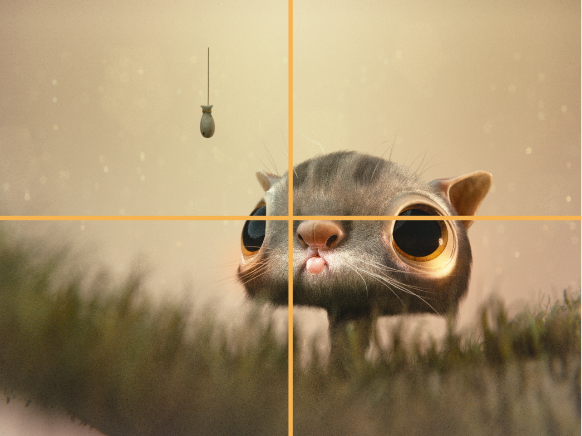
\includegraphics{decou_re}}
\caption{Rendering with inbalanced times}
\label{decou_re}
\end{figure}



\section{An adaptive approach} \label{TwoPhases}

\subsection{Principle}

\iffalse
Explain that we will make a workload estimation and then we will compute the 
balanced decomposition

Picture that summarizes the approach
\fi
Our approach reduces the rendering time in a way similar to doing the trade-off between exploration and exploitation. Our approach procedes as follows: firstly, we do a fine-level estimation of rendering time of different parts of the image based on a fine-level splitting of it using a small number of samples and later we will show that this estimation is good enough; secondly, according to this estimation, we propose an splitting which can approximate the optimum rectangle solution. Fig.~\ref{grid} and Fig.~\ref{decou_irre} demonstrate these two steps. Our goal is to have the sum of estimation time and rendering time lower than the rendering time of a regular splitting as much as possible. 

\begin{figure}[htbp]
\centerline{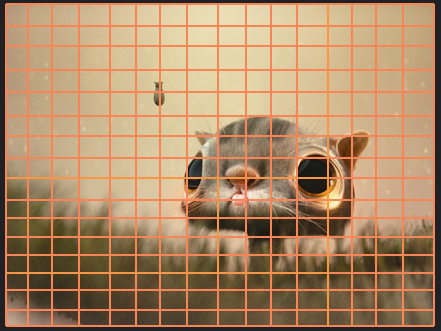
\includegraphics{grid}}
\caption{Fine-level rendering time estimation: after this step, we can obtain the rendering time of the small sub-images}
\label{grid}
\end{figure}

\begin{figure}[htbp]
\centerline{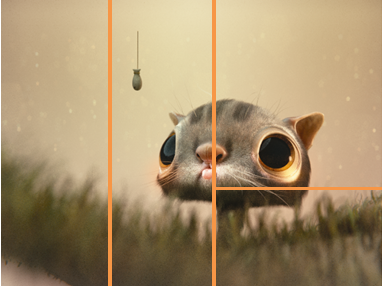
\includegraphics{decou_irre}}
\caption{In the second step, we use a heuristic algorithm to find the optimal solution}
\label{decou_irre}
\end{figure}

\subsection{Implementation model}

\iffalse
Explain how the principle is implemented with Q.ware. Mention software 
components to develop.

Explain the limits of the model (the scheduling will not necessarily be optimal ...)
\fi

The estimation is first implemented in a processor by launching rendering to the given image in the software Blender using a small number of samples. Blender renders an image on the level of small sub-images. We make use of this and retreive a good enough estimation of the rendering time for the case of a large number of samples of these fine-level sub-images. With this estimation of rendering time, we execute a heuristic algorithm to approximate the optimal solution to the problem. Then we send the parameters which can define the splitting to Q.ware, which dispatches the rendering tasks to processors. When the rendering of sub-images is finished, we retrieve them and compose them together using the software ImageMagick.

Several factors may affect the efficiency of the model. Firstly, the scheduling in Q.ware may not be optimal and the resulted rendering times may not be as balanced as expected. Secondly, when the regular splitting fits well the pattern of the image, the model adds additional cost for the rendering task compared with the regular splitting model. 





\subsection{Workload estimation}

Define the problem (given a piece of an image, we want to know what is the runtime of the rendering)

Define the method to solve the problem (Fine grain decomposition of the image and then 
make a noisy rendering to estimate the duration)

Say why the method could work (Monte Carlo theory ...)

Say what are the limits: 

 - what is the noise level we consider for rendering? This is the 

old dilema between exploration and exploitation.
 - What is the right decomposition grain?


\subsection{Load balancing}

Define the problem (we have an estimation of a fine grain decomposition, what is the best 
partitioning in N rectangles?)

Recall that it is a classical NP hard problems

Say that there exist several algorithms. But they are not efficient to capture irregular decompositions.

Present the Tetris algorithm as a solution for more irregular decompositions

Put the pseudo code

\section{Experimental evaluation} \label{Experimental}

Present the dataset

Results of the file prepared for the Blender conf

Analyze the strong and weak points of Tetris

Strong: 
Explain that in general tetris is more interesting when we have more rectangles 
or when the optimal decomposition has a too irregular shape.
 Show some shapes (decomposition) that cannot be captured by the other algorithms. 

Weak points: Show that we tend to have smaller rectangles at the top.
Illustrate on an example.

Recommend the perfect image for Tetris...


\section{Related works} \label{RelatedWorks}

Existing works on workload estimation.

Existing works on partitioning.

\section{Conclusion} \label{Conclusion}


\def\IEEEbibitemsep{.1pt}
\bibliographystyle{./IEEEtran}
\bibliography{hpcs2018}

\end{document}
